\section{Mechanics}
\label{sec:dp-pds-mechanics}

\subsection{\dshort{pmt} Support Structure}
\label{subsec:dp-pds-mechanics-pmtsupport}

A uniform array of \dpnumpmtch cryogenic Hamamatsu R5912-MOD20 \dwords{pmt}, below the transparent cathode structure, will be fixed on the membrane floor in the areas between the membrane corrugations. The arrangement of the \dwords{pmt} accommodates the cryogenic piping on the membrane floor, and other elements installed in this area.

The mechanics for the attachment of the \dwords{pmt} were carefully studied. The \dword{pmt} buoyancy must be counteracted while avoiding stress to the \dword{pmt} glass due to differentials in the thermal contraction between the support and the \dword{pmt} itself. The attachment is done via a stainless steel support base point-glued to the membrane via four adhesive injection holes. The weight of the support and \dword{pmt} (approximately \SI{7}{\kg}) exceeds the buoyancy force of the system. Given the large standing surface of the stainless steel plate, these supports also ensure stability against possible lateral forces acting on the \dwords{pmt} due to the liquid flow. Figure \ref{fig:dppd_3_2} shows the \dword{pmt} with its support base attached to the bottom of the \dword{pddp} cryostat.

%\begin{dunefigure}[Cryogenic Hamamatsu R5912-MOD20 \dword{pmt} %fixed on the membrane floor.]{fig:dppd_3_2}
%{Cryogenic Hamamatsu R5912-MOD20 \dword{pmt} fixed on the membrane floor, with the optical fiber of the calibration system.}
%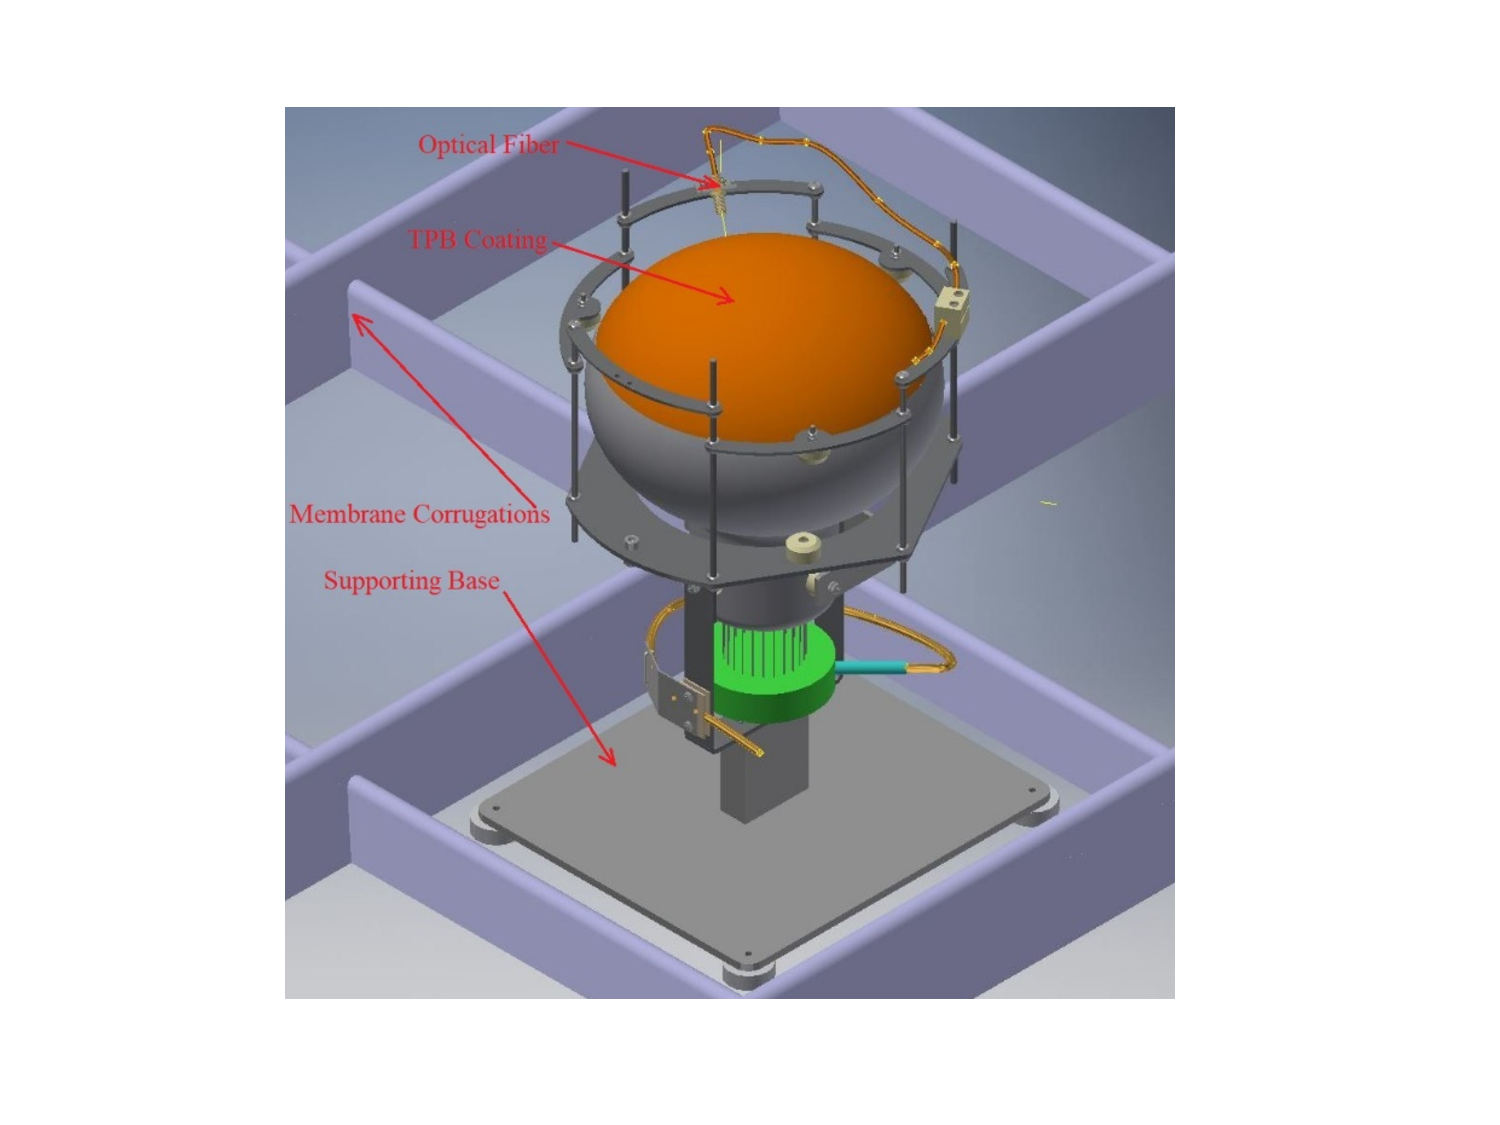
\includegraphics[width=0.42\textwidth]{dppd_3_2}
%\end{dunefigure}

\begin{dunefigure}[Picture of the Hamamatsu R5912-MOD20 \dword{pmt} fixed on the membrane floor of \dword{pddp}.]{fig:dppd_3_2}
{Picture of the cryogenic Hamamatsu R5912-MOD20 \dword{pmt} fixed on the membrane floor of \dword{pddp}. The optical fiber of the calibration system is also visible.}
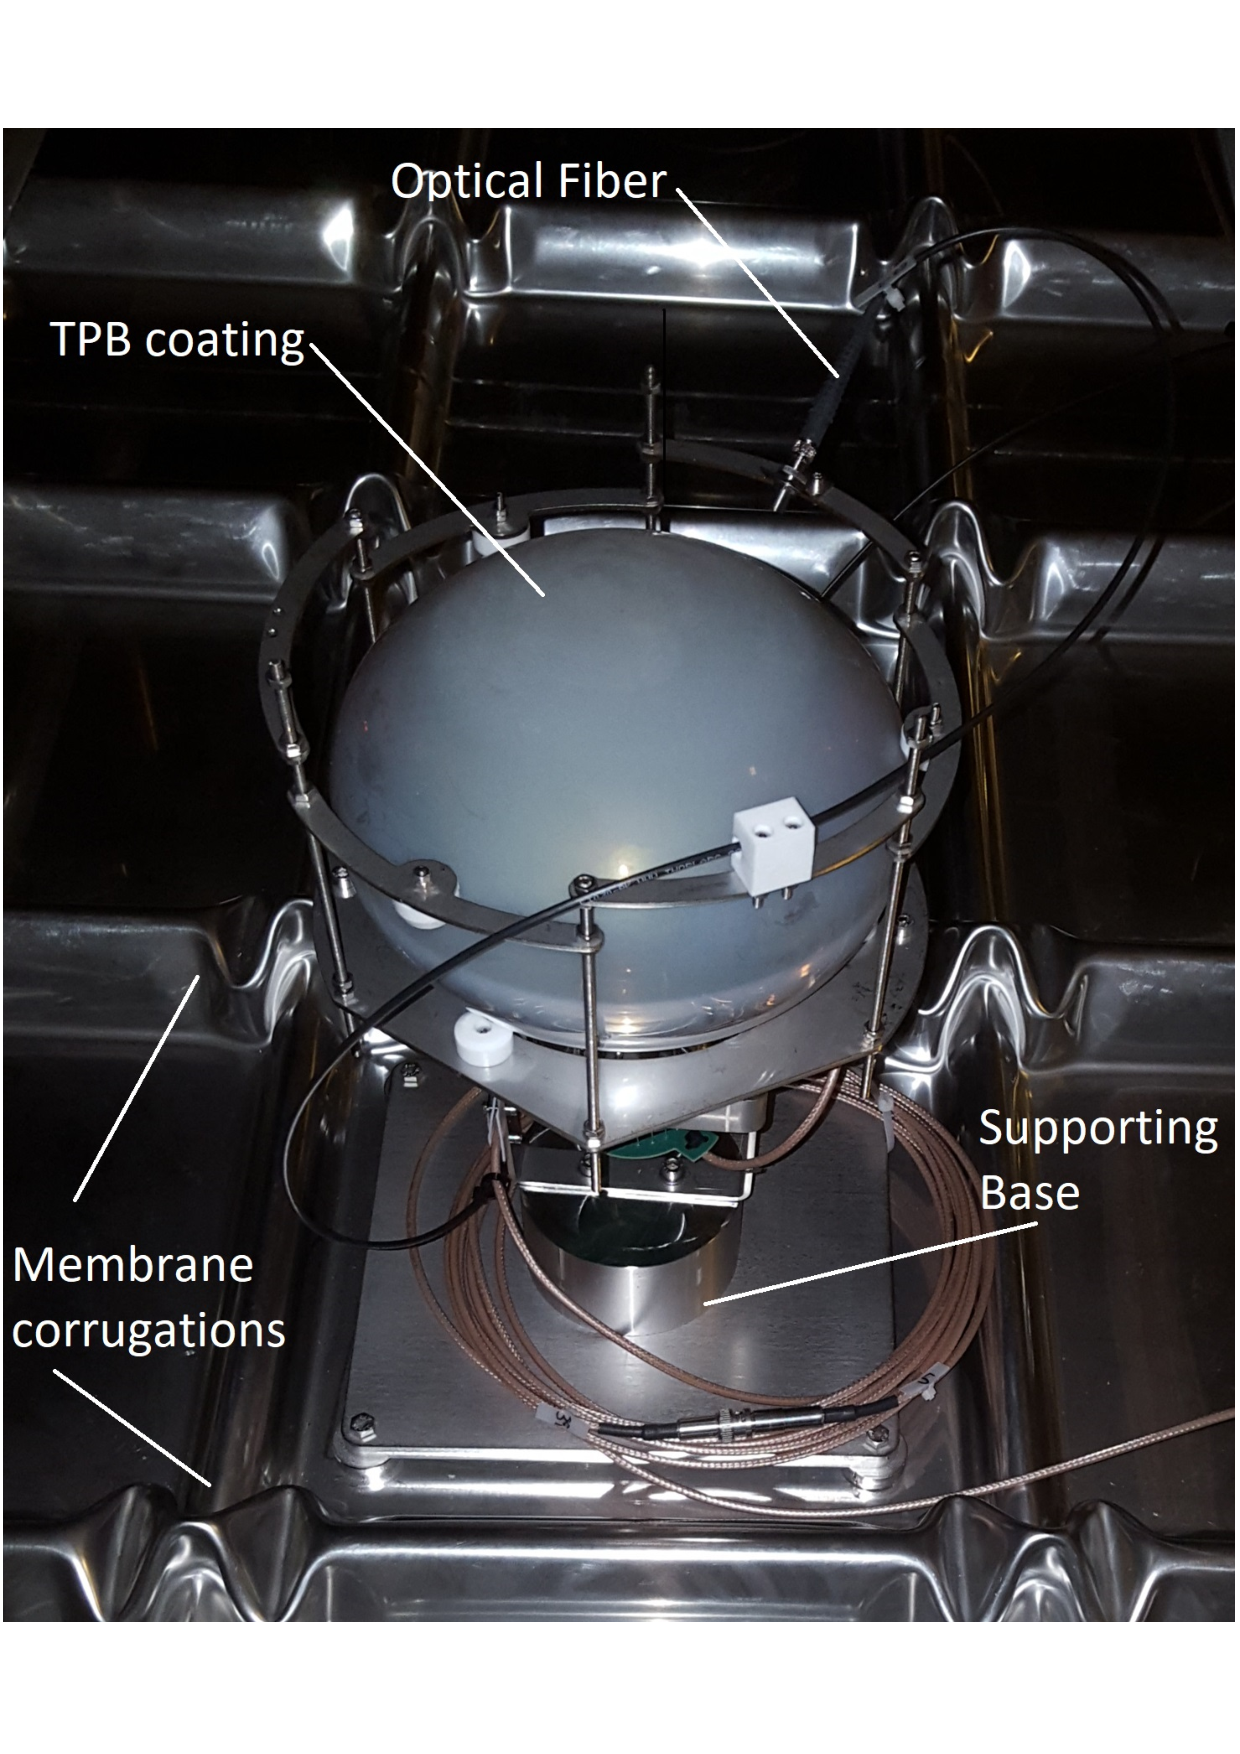
\includegraphics[width=0.42\textwidth]{dppd_3_n2}
\end{dunefigure}

%\fixme{Update Fig.~\ref{fig:dppd_3_2} of PMT support structure.}

%The \dword{hv} and \dual \dword{pds} consortia is studying an alternative to the table-like assembly of the ground grid: the concept of individual ground grids for each \dword{pmt}. In this option, the grids would be mechanically attached to the support structure. This will increase the acceptance of the \dwords{pmt} at larger angles.

The support frame structure mainly comprises \num{304}L stainless steel with some small Teflon (PTFE) pieces assembled by A4 stainless steel screws that minimize the mass while securing the \dword{pmt} support to the cryostat membrane. The design %was done taking 
takes into account the shrinking of the different materials during the cooling process to avoid breaking the \dword{pmt} glass.
Over-pressure tests were carried out for \dword{pddp}, and further tests ensure correct performance under pressure. An individual \dword{pmt} mount has been designed and tested in the  \dword{wa105} prototype~\cite{Zambelli:2017dkg}, and the same design is used for \dword{pddp}.

Installation of an individual ground grids mechanically attached to the \dword{pmt} support structures is also under consideration by the \dword{hv} and \dual \dword{pds} consortia (See Appendix~\ref{sec:dp-pds-appendix-grid}).

%%%%%%%%%%%%%%%%%%%%%%%%%%%%%%%%%%%%%%%%%%%%%%%%%%%%%%%%%%%%%%%%%%%

\subsection{Reflector/\dshort{wls} Panel Assemblies}
\label{subsec:dp-pds-mechanics-reflectors}

The reflector/\dword{wls} panels that will be mounted on the inner surface of the \dword{fc} will be \SI{1}{\mm} thick \SI{93}{\cm} $\times$ \SI{93}{\cm} G10/FR4 plates, with the central \SI{91}{\cm} (H) $\times$ \SI{93}{\cm} (W) area laminated with reflective foil, which is coated with \dword{tpb} (see Fig.~\ref{fig:dppd_reflective_panel}). The panels will be supported by G10/FR4 support bars. Six horizontal bars of \SI{199}{\cm} (three at the front and three at the back), six vertical bars of \SI{186}{\cm} (all at the back) and four reflector/\dword{wls} panels will form a unit reflector/\dword{wls} panel assembly to be mounted on the \dword{fc}. The panels will be sandwiched between the horizontal support bars along the non-laminated edges. Six vertical bars will be placed on the side of the panels without the reflective coating, aligning the holes. The structure will then be assembled by placing \num{24} screws.

The horizontal support bars will be attached to the FRP I-beams of the \dword{fc}, which are spaced \SI{2}{\m} apart, by stainless steel screws. One end of the bar will be tightly screwed, while the other loosely to allow motion due to differential thermal contractions. Figure \ref{fig:dppd_reflective_panel_support} shows sketches of the horizontal support bars with one of the two screw holes elongated to allow the support bar movement on the mounting screw.

\begin{dunefigure}[Sketches of the reflector/\dword{wls} panel assembly horizontal support bars.]{fig:dppd_reflective_panel_support}
{Sketches of the reflector/\dword{wls} panel assembly horizontal support bars (not to scale). (a) The top and bottom bars, (b) the middle bar, (c) the extended top and bottom bars to be mounted on the end submodules of the \dword{fc} super-modules, and (d) the special extended top and bottom bars to be mounted on the end submodules of the corner \dword{fc} side wall super-modules.}
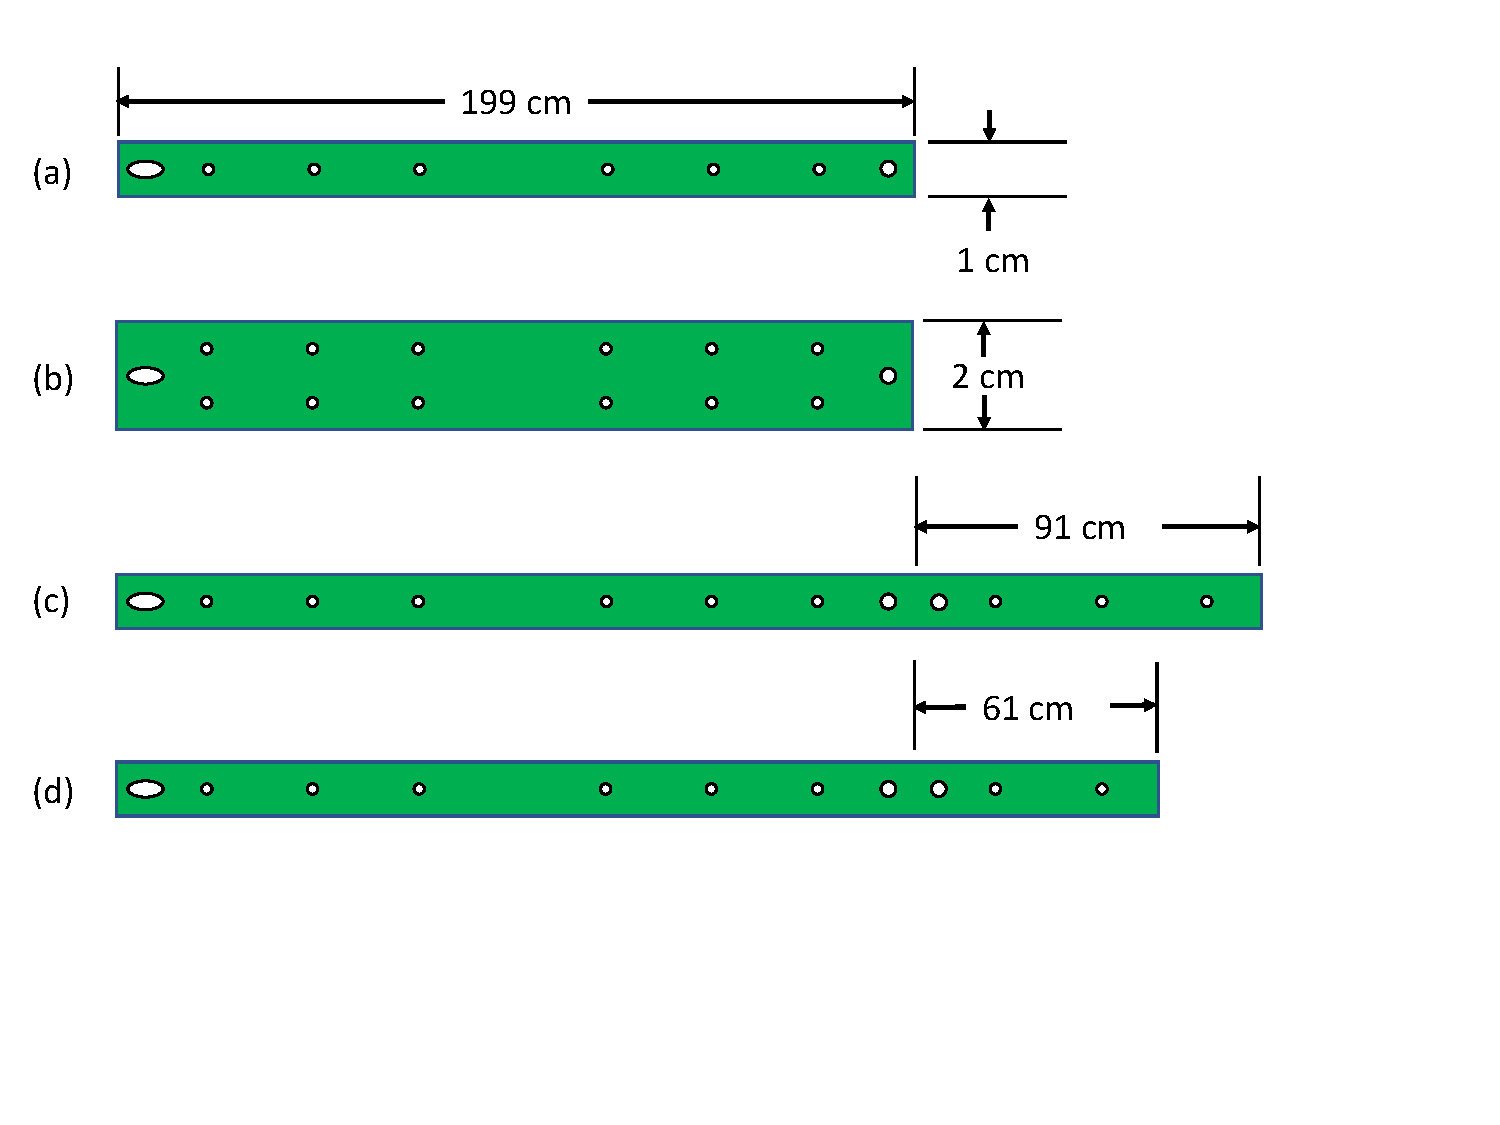
\includegraphics[width=0.65\textwidth]{dppd_reflective_panel_support}
\end{dunefigure}

The reflector/\dword{wls} panel assemblies at the inter-super-module areas will have extended structures: \SI{260}{\cm} (W) $\times$ \SI{186}{\cm} (H) for the corner side wall \dword{fc} sub-modules to accommodate the \num{2.4} degree tilt of the end walls, and \SI{290}{\cm} (W) $\times$ \SI{186}{\cm} (H) for all other \dword{fc} sub-modules at the intersection of two \dword{fc} super-modules. The extended assemblies will house \num{6} reflector/\dword{wls} panels, two of them in an extended part which is not supported at the end. Figure \ref{fig:dppd_reflective_panel_support} (c) shows the sketch of the support bar to be installed at the end submodules of the \dword{fc} super-modules except the end submodules of the corner \dword{fc} side wall super-modules of which the corresponding horizontal support bar is shown in Fig.~\ref{fig:dppd_reflective_panel_support} (d). The special extended assemblies to be installed at the end submodules of the corner side wall super-modules will be \SI{30}{\cm} shorter than the regular extended assemblies to accommodate the approximately \SI{25}{\cm} approach of the end walls at middle drift distance (\SI{6}{\m}).

Figure \ref{fig:dppd_reflective_panel_onFC} shows inside (left) and outside (right) sketches of a unit reflector/\dword{wls} assembly. The blue bars are the I-beams of the \dword{fc}, the dark green bars are the horizontal and vertical support bars of the reflector/\dword{wls} panel assembly. The grey surfaces are the \dword{tpb} coatings on the panels. The vertical and horizontal gaps between the reflector/\dword{wls} panels allow liquid flow. 

\begin{dunefigure}[Sketches of the inside and outside views of a partial \dword{fc} submodule with a reflector/\dword{wls} panel assembly.]{fig:dppd_reflective_panel_onFC}
{Sketches of the inside with the reflective/\dword{wls} coating (left) and outside without the reflective/\dword{wls} coating (right) views of a partial \dword{fc} submodule with a reflector/\dword{wls} panel assembly. The blue bars are the FRP I-beams of the \dword{fc}. The dark green bars are the horizontal and vertical support bars. The grey surfaces are the \dword{tpb} coatings on the panels.}
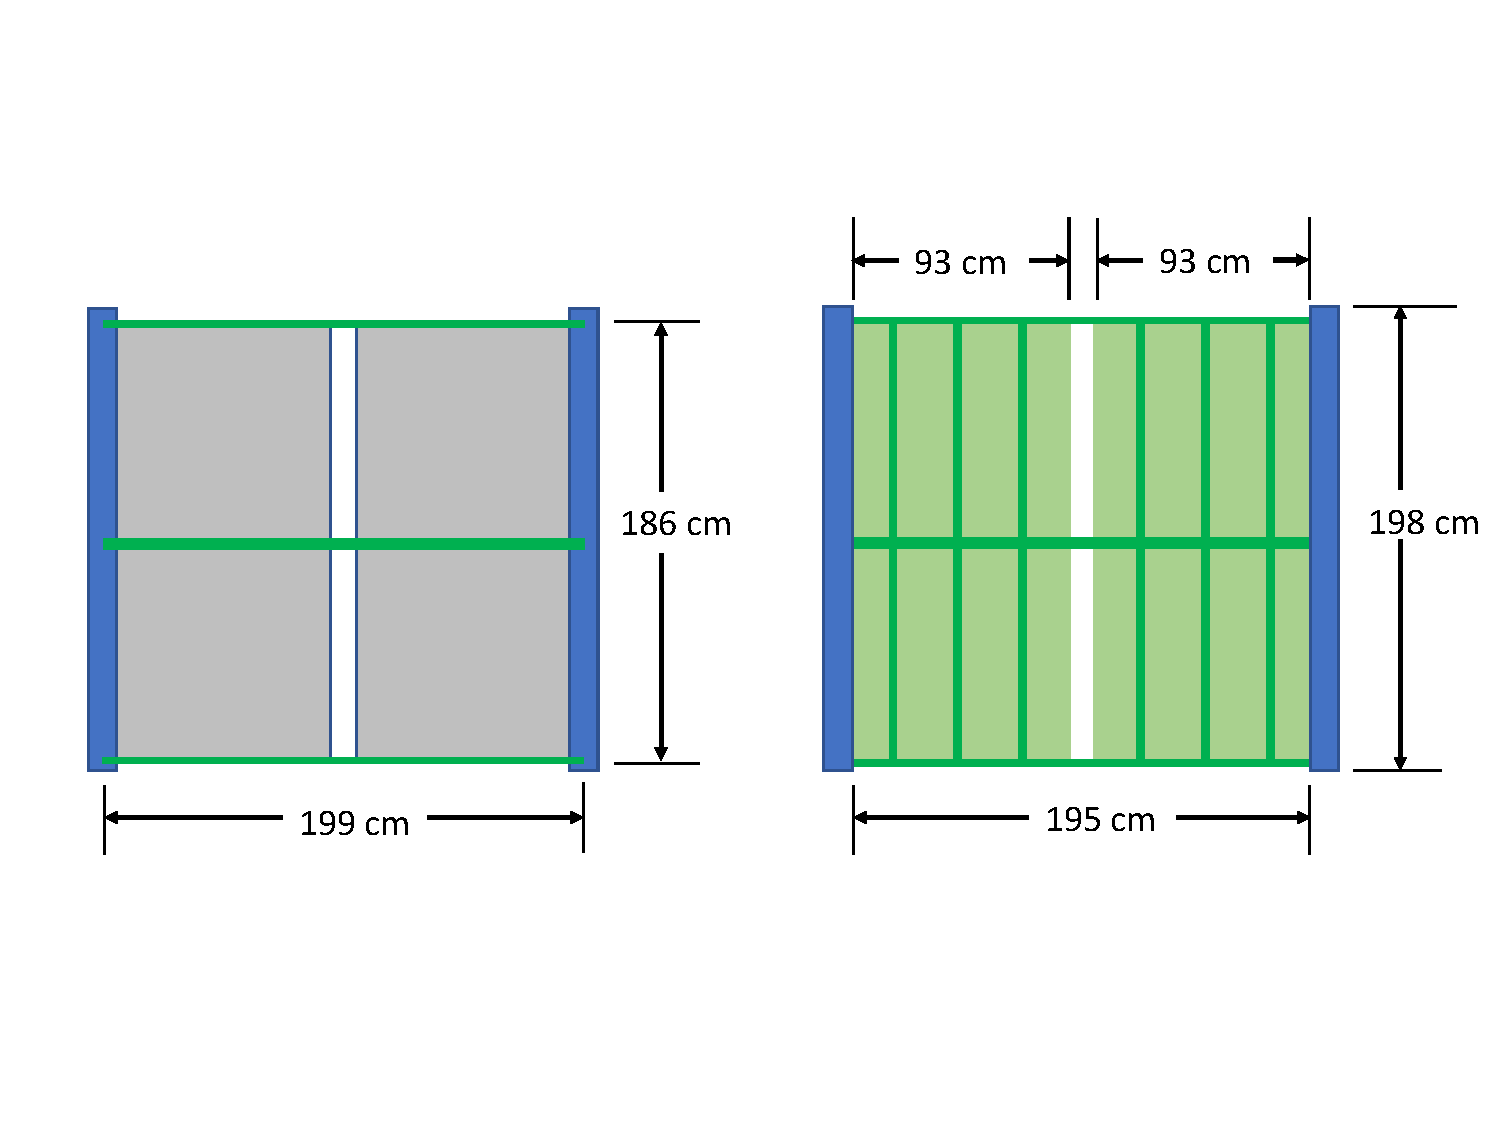
\includegraphics[width=0.8\textwidth]{dppd_reflective_panel_onFC}
\end{dunefigure}